\documentclass{standalone}

% Plotting
\usepackage{tikz}
\usetikzlibrary{decorations.markings}
\usetikzlibrary{calc}
% quantikz breaks tikz-cd, see https://tex.stackexchange.com/questions/618330/quantikz-breaks-spacing-in-tikz-matrices-tikz-cd
%\usetikzlibrary{quantikz}
\usetikzlibrary{cd}
\usepackage{pgfplots}

\usepackage{simpler-wick}
\usepackage{physics}

\usepackage{amsmath}
\usepackage{mathtools}

\begin{document}
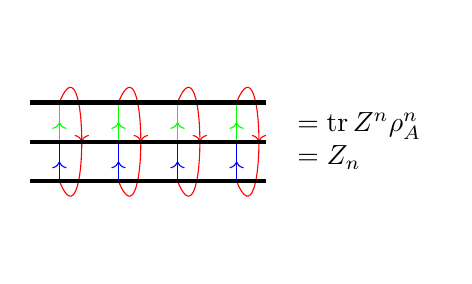
\begin{tikzpicture}[xscale=1.5,decoration={
    markings,
    mark=at position 0.5 with {\arrow{>}}}]

    \foreach \i in {0.25,0.75,...,1.75} {
        \draw[blue, postaction={decorate}] (\i, 0) -- (\i, 0.5);
        \draw[green, postaction={decorate}] (\i, 0.5) -- (\i, 1);
        \draw[red, postaction={decorate}] (\i, 1) to[out=75, in=-75, looseness=2.5] (\i, 0);
    }
    \draw[ultra thick] (0,0) -- (2,0);
    \draw[ultra thick] (0,0.5) -- (2,0.5);
    \draw[ultra thick] (0,1) -- (2,1);
    \draw (2,0.5) node[anchor=west] {$\begin{array}{l}
        {}= \tr Z^n \rho_A^n \\
        {}= Z_n
    \end{array}$};
\end{tikzpicture}
\end{document}